\documentclass[11pt]{article}

\usepackage{amssymb, amsmath, amsthm}
\usepackage{graphicx} 
\usepackage{wrapfig}

\title{ Homework 1 }
\author{ Jacob Hurst }
\date{\today}

\begin{document}

\maketitle
\clearpage

\section{Question 1}
\subsection{On inputs of size n, the number of clock cycles needed by Algorithm A and Algorithm B are given by $ 32nlog(n) $ and $ 2n^2 $, respectively. Determine a value, x, such that Algorithm A performs better than algorithm B whenever n $\geq$ x. }

\begin{wrapfigure}{l}{0.5\textwidth}
  \begin{center}
    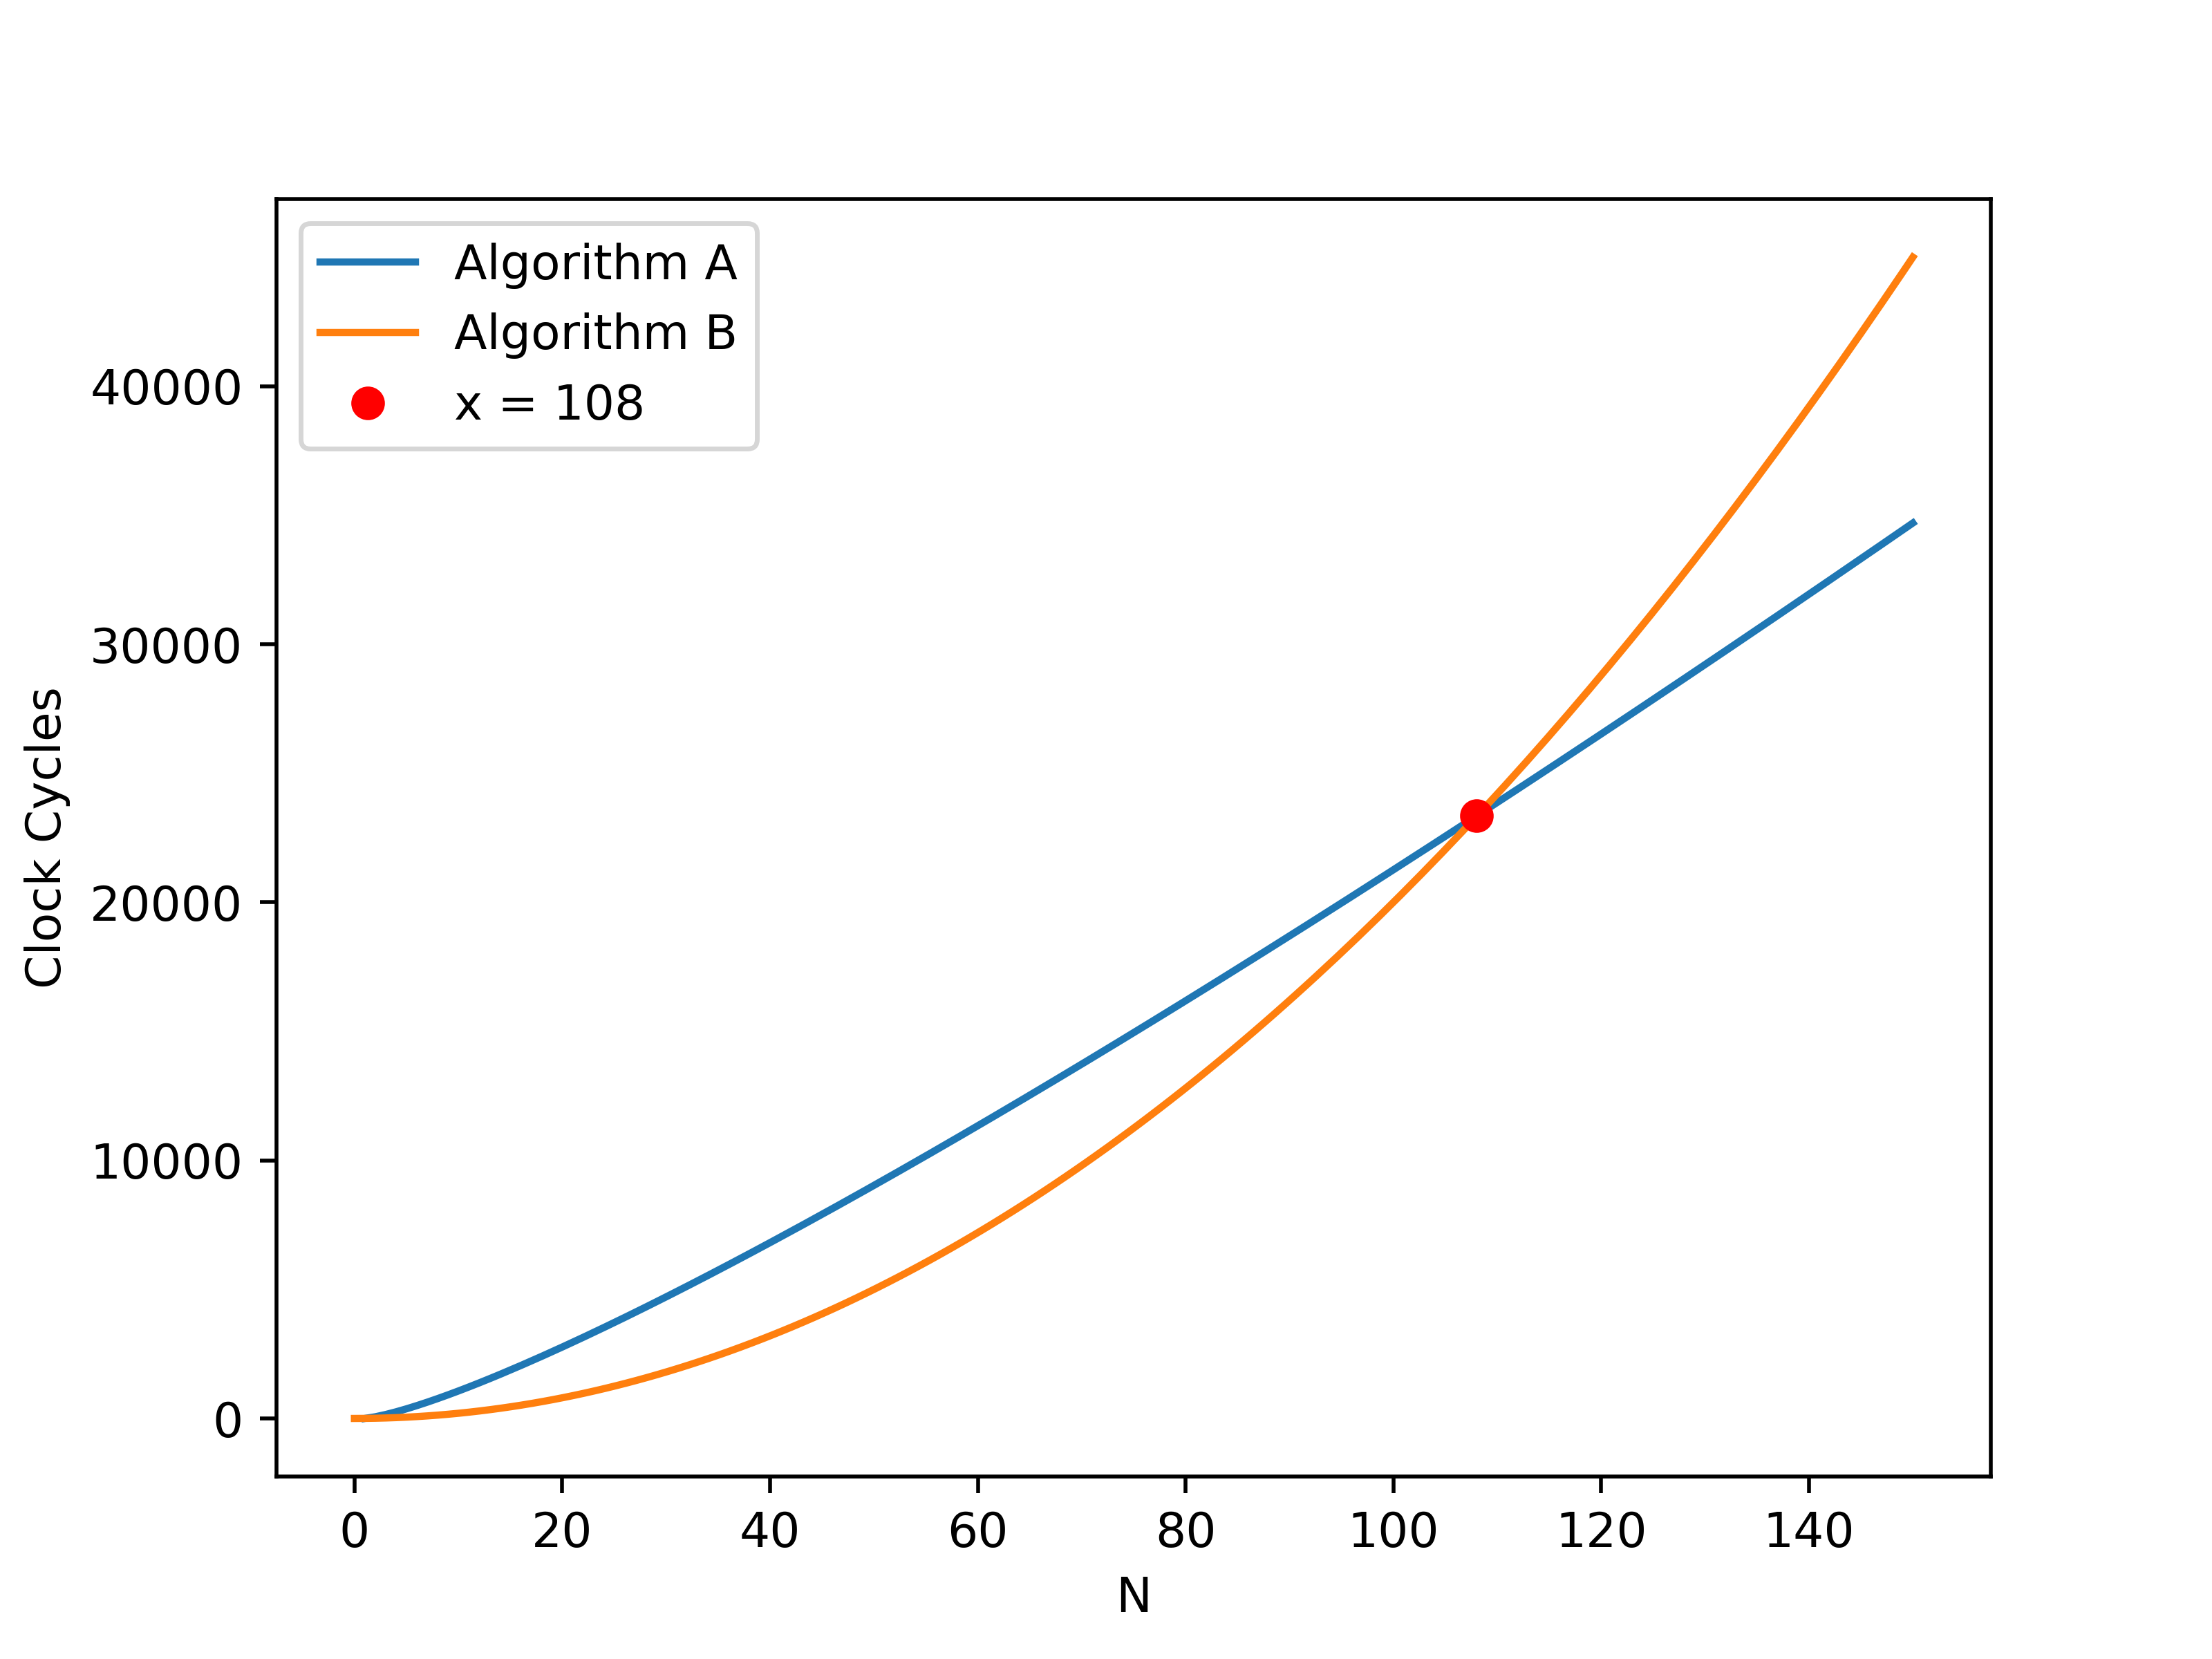
\includegraphics[width=0.48\textwidth]{q1.png}
  \end{center}
  \caption{Plot of Algorithms}
\end{wrapfigure}

 Plotting the given functions clock cycles as n increases from 0 to 150,
 we may observe that Algorithm A and B intersect at the point n = 108. If we select x to be 108, we can compare performance of Algorithm A and B at 107, 108, and 109. \\$ Algorithm A:\\32*107*log(107) = 23,078\\32*108*log(108) = 23,328\\32*109*log(109) = 23,614\\Algorithm B:\\2*107^2 = 22,898\\2*108^2 = 23,328\\2*109^2 = 23,762$. \\\\Notice that Algorithm A's clock cycles are greater than Algorithm B's clock cycles at x = 107, equivalent at x = 108, and less than x = 109. Therefore, when n $\geq$ 108, Algorithm A performs better than Algorithm B. 
\\\\Alternatively, we may solve for $ 32*n*log(n) < C*2*n^2 $ where C is some constant, and find $log(n) < (C/16)*n$. If $C=16$, we have $log(n) < n$ which is true for all $n > 1$.

\section{Question 2}
\subsection{On inputs of size n, the number of clock cycles needed by Algorithm A and Algorithm B are given by $ 50n^2 $ and $ 2n^3 $, respectively. Determine a value, x, such that Algorithm A performs better than Algorithm B whenever n $\geq$ x. }

Setting the given functions equal to eachother, we have $50*n^2 = 2*n^3$. We can solve for this and find a point of intersection. $50*n^2 / 2*n^3 = 1 \rightarrow 25/n = 1 \rightarrow n = 25$. We can compare the performance of Algorithm A and B at 24, 25, and 26. \\$Algorithm A:\\50*24^2 = 28,800\\50*25^2 = 31,250\\50*26^2 = 33,800\\Algorithm B:\\2*24^3=27,648\\2*25^3=31,250\\2*26^3=35,152\\$\\Notice that Algorithm A's clock cycles are greater than Algorithm B's clock cycles at x = 24, equivalent at x = 25, and less than x = 26. Therefore, when n $\geq$ 25, Algorithm A performs better than Algorithm B.

\section{Question 3}
\subsection{Express the function $ 1 + 2 + ... + log(N) $ in big-O notation (answer must not include ellipsis).}

Recall $\sum_{i=1}^{n} i = 1 + 2 + ... + n = n(n +1)/2$. \\\\Using this same, summation we can substitute n for log(N) to get $\sum_{i=1}^{log(N)} i = 1 + 2 + ... + log(N) = log(N)(log(N)+1)/2 = (log^2(N)+log(N))/2$. \\\\In big-O notation, this can be written as $O((log^2(N)+log(N))/2) \rightarrow O(log^2(N)+log(N)) \rightarrow O(log^2(N))$

\section{Question 4}
\subsection{Suppose you have algorithms with running times (a) $ n^2 $, (b) $ n^3 $, (c) $ 100n^2 $, (d) $ nlog(n) $, (e) $ 2^n $, (f) $ n \sqrt n $. How much slower does each of these algorithms get when you (1) double the input size, n, or (2) increase the input size by 1?}

a) $ n^2 $\\
Doubling our input size gives us $ f(2n)=(2n)^2=4n^2 $ running time. Our running time is increased by a factor of 4 when our input size is doubled.\\
Adding 1 to input size gives us $ f(n+1)=(n+1)^2=n^2+2n+1 $ running time. Our running time is increased by $2n+1$.\\\\
b) $ n^3 $\\
Doubling our input size gives us $ f(2n)=(2n)^3=8n^3 $ running time. Our running time is increased by a factor of 8 when our input size is doubled.\\
Adding 1 to input size gives us $ f(n+1)=(n+1)^3=n^3+3n^2+3n+1 $ running time. Our running time is increased by $3n^2+3n+1$.\\\\
c) $ 100n^2 $\\
Doubling our input size gives us $ f(2n)=100(2n)^2=100*4n^2=400n^2 $ running time. Our running time is increased by a factor of 4 when our input size is doubled.\\
Adding 1 to input size gives us $ f(n+1)=100(n+1)^2=100(n^2+2n+1)=100n^2+200n+100 $ running time. Our running time is increased by $ 200n+100 $.\\\\
d) $ nlog(n) $\\
Doubling our input size gives us $ f(2n)=2nlog(2n)=2n((log(n)/log(2)) + 1)=2n(log(n)+1)=2nlog(n)+2n=nlog(n)+nlog(n)+2n $ running time. Our running time is increased by $nlog(n) + 2n$.\\
Adding 1 to input size gives us $ f(n+1)=(n+1)log(n+1)=(n+1)(log(n) + 1/n)= nlog(n) + 1 + log(n) + 1/n $ running time. Our running time is increased by $1 + log(n) + 1/n$.\\\\
e) $ 2^n $\\
Doubling our input size gives us $ f(2n)=2^{2n}=4^n $ running time. Our running time is increased from $2*2*...2*2 $(n terms) to $4*4*...4*4 $(n terms) which is a significantly longer running time. Example: $n=2: 2^2 = 4,  4^2 = 16$.\\\\
Adding 1 to input size gives us $ f(n+1)=2^{n+1}=2*2^n $ running time. Our running time is doubled when our input size is increased by 1.\\\\
f) $ n \sqrt n $\\
Doubling our input size gives us $ f(2n)=2n \sqrt {2n} = 2 \sqrt 2 n \sqrt n$ running time. Our running time is increased by a factor of $2 \sqrt 2$.\\
Adding 1 to input size gives us $ f(n+1)=(n+1) \sqrt {n+1} = n \sqrt {n+1} + \sqrt {n+1} $ running time. Our running time is increased by approximately $1 + \sqrt {n+1}$.\\

\section{Question 5}
\subsection{Suppose we have a deterministic version of QuickSort that, on an array of size n, always chooses the element at index Floor($ n/2 $) as its pivot. What is the running time of this version of QuickSort on an input array that is already correctly sorted?}

The runtime of the standard QuickSort algorithm depends on how balanced its partitions are. The balance of its partitions is determined by its pivot element. If the pivot element is the smallest or largest in the array, then one of the two partitions will contain $n-1$ of the elements. If the pivot element is the median of the list, then each partition will contain $n/2$ elements. The best case of standard QuickSort occurs when the median is continually selected as the pivot element $\rightarrow \Theta (nlog(n)) $ since each of the n steps partitions into two equally sized subsets (log(n)).\\\\If our input is correctly sorted and the pivot is always selected to be Floor($n/2$), then the median element will be selected on each step of partitioning the array. This means that our deterministic QuickSort with pivot selected as Floor($n/2$) will have a running time (on correctly sorted input) of $nlog(n)$.

\section{Question 6}
\subsection{Consider the same version of QuickSort from Question 5. Describe the kind of sequence that would cause this algorithm to run in $ \Omega (n^2) $ time.}

If on each partitioning, the pivot, Floor($n/2$), happens to be the smallest or largest element in the array, we will have $ \Omega (n^2) $ time. A sequence like this would result in each of the n partition levels containing one partition with $n-1$ elements and the other with 0 elements $\rightarrow \Omega (n(n-1)) \rightarrow \Omega (n^2 - n) \rightarrow \Omega (n^2)$. Example: A[4,9,3,8] pivot=9 $\rightarrow$ A[4,3,8] [9] pivot=3 $\rightarrow$ A[4,8] [3] pivot 4 $\rightarrow$ A[8] [4].

\end{document}  